%% ==============================
\chapter{Methoden der Dimensionsreduktion}
\label{ch:MethodenDerDimRed}
%% ==============================

Nachdem wir nun die Motivation und Idee hinter der Dimensionsreduktion in \chapref{ch:Enleitung} und die mathematische Formulierung
in \chapref{ch:Dimensionsreduktion} allgemein angeschaut haben,
werden nun einige Methoden zur Dimensionsreduktion vorgestellt.

In jüngster Zeit haben vor allem verschiedenste Varianten von neuronale Netzen einen hohen Grad an Aufmerksamkeit durch bahnbrechende Errungenschaften in Gebieten der Spracherkennung oder \textit{Computer Vision} erlangt. Fraglich ist, ob diese neuen Algorithmen auch auf dem Bereich der Dimensionsreduktion einen entscheidenden Fortschritt gemacht haben. Deshalb unterteilen wir die Algorithmen in \textit{traditionelle}
und \textit{moderne} Methoden, um diese später in \chapref{ch:Vergleich} gegenüberstellen zu können. Mit traditionellen Methoden
sind statistische Methoden wie die Hauptkomponentenanalyse (\subsecref{ch:MethodenDerDimRed:traditionell:PCA}) oder andere etablierte
Methoden der Dimensionsreduktion gemeint, wohingegen moderne Methoden auf neuere Entwicklungen wie neuronale Netze und die Varianten davon abzielt. Allerdings ist hier aus jeder Kategorie nur eine kleine repräsentative Auswahl getroffen worden. Weitere wichtige Algorithmen, die hier nicht vorgestellt werden können sind beispielsweise \dots \todo{Nachweise für Algorithmen + aufzählen}.

\section{Traditionelle Methoden}
\label{ch:MethodenDerDimRed:traditionell}

Zuerst widmen wir uns den traditionellen Methoden der Dimensionsreduktion.
Dazu gehören die \newterm{Hauptkomponentenanalyse} (engl. \textit{principal components analysis} (PCA)) in \subsecref{ch:MethodenDerDimRed:traditionell:PCA},
die nichtlineare Erweiterung der
Hauptkomponentenanalyse (\subsecref{ch:MethodenDerDimRed:traditionell:kPCA})
und die für die Visualisierung sehr verbreitete Methode \newterm{t-distributed stochastic neighborhood embedding} (t-SNE) in \subsecref{ch:MethodenDerDimRed:traditionell:t-SNE}.

%% ==============================
\subsection{Principal Component Analysis}
\label{ch:MethodenDerDimRed:traditionell:PCA}
\nomenclature[Z]{PCA}{Principal Component Analysis}

Principal Component Analysis ist \textit{die} Methode der Dimensionsreduktion und wurde erstmals von \textcite{Pearson.1901} und Hotelling 1933\addref entwickelt. Trotz des mittlerweile relativ hohen Alters ist die Hauptkomponentenanalyse immer noch aufgrund der simplen Anwendbarkeit oft die erste Wahl einer Dimensionsreduktionsmethode. Im Folgenden möchte ich kurz auf die zentrale Idee und Motivation (\ref{ch:MethodenDerDimRed:traditionell:PCA:Grundidee}) der Hauptkomponentenanalyse, sowie die mathematische Herleitung der sogenannten \newterm{Hauptkomponenten} (Unterabschnitte \ref{ch:MethodenDerDimRed:traditionell:PCA:Definition} und \ref{ch:MethodenDerDimRed:traditionell:PCA:HerleitungPC}) eingehen.


\subsubsection{Grundidee}
\label{ch:MethodenDerDimRed:traditionell:PCA:Grundidee}
Die zentrale Idee der Hauptkomponentenanalyse ist die Transformation des Koordinatensystems in einer möglichst \textit{verlustfreien} Art und Weise. Verlustfrei bedeutet im Kontext der Hauptkomponentenanalyse, dass möglichst viel Variation in den Daten erhalten bleiben soll \parencite[vgl.][1]{Jolliffe.2002}. Möchte man dann die Dimension von $D$ auf die intrinsische Dimension $d$ reduzieren wählt man einfach die \textit{ersten} $d$ Hauptkomponenten. Was diese Hauptkomponenten sind, werden wir im Folgenden genauer sehen.

\subsubsection{Definition der Hauptkomponenten}
\label{ch:MethodenDerDimRed:traditionell:PCA:Definition}
Wir haben also als Ausgangsbasis einen $D$-dimensionalen Zufallsvektor $\rvect{x} = \tr{(\rv{x}_1, \ldots, \rv{x}_D)}$ mit $\Exp[\rvect{x}] = \vect{0}$ und unser Ziel ist es, eine $k$-dimensionale Repräsentation $\rvect{y} = \tr{(\rv{y_1},\ldots,\rv{y}_k)}$ zu erhalten. Idealerweise setzt man $k$ auf die intrinsische Dimension $d$ von $\rvect{x}$, hier soll jedoch nur der Fokus auf die allgemeine Dimensionsreduktion gelegt werden. Wir drücken also $\rvect{y}$ als eine Linearkombination des ursprünglichen hochdimensionalen Vektors $\rvect{x}$ wie folgt aus:
\begin{equation}
	\rv{y}_i = \tr{\vect{a}_i} \rvect{x} = \sc{a}_{i1} \rv{x}_1 + \cdots + \sc{a}_{iD} \rv{x}_D
	\quad i = 1,\ldots,k
\end{equation}
wobei $\vect{a}_i$ die \newterm{Koeffizienten} (auch: Ladungen) der $i$-ten Hauptkomponente sind \parencite[vgl.][2]{Jolliffe.2002}. Die Anzahl $k$ der Hauptkomponenten bestimmt den Grad der Dimensionsreduktion, kann jedoch beliebig zwischen $1 \leq k \leq D$ gewählt werden.\footnote{Der Grenzfall $k = D$ wird oft für eine Anonymisierung des Datensatzes mit personenbezogenen Daten verwendet. Beispielsweise kann so bei Finanztransaktionen der Datensatz mithilfe von PCA vorverarbeitet (\textit{Preprocessing}) und erst dann veröffentlicht werden.}

\subsubsection{Herleitung der Hauptkomponenten}
\label{ch:MethodenDerDimRed:traditionell:PCA:HerleitungPC}
Wir betrachten nun zunächst lediglich die \textit{erste} Hauptkomponente $\tr{\vect{a}_1} \rvect{x}$ und erinnern uns daran, dass wir wie in \subsecref{ch:MethodenDerDimRed:traditionell:PCA:Grundidee} erwähnt möglichst viel Variation von $\rvect{x}$ erhalten möchten. Daher maximieren wir die erste Hauptkomponente so, dass die Varianz maximal wird:
\begin{equation}
	\label{eq:PCA-Optimierungsproblem}
	\max_\vect{a_1} \Var \left( \tr{\vect{a}_1} \rvect{x} \right) = \max_\vect{a_1} \tr{\vect{a}_1} \mat{\Sigma} \vect{a}_1
\end{equation}
wobei $\mat{\Sigma}$ die Kovarianzmatrix von $\rvect{x}$ ist. Dieses Maximierungsproblem ist jedoch nach oben unbeschränkt, weshalb man zusätzlich die Bedingung
\begin{equation}
	\norm{ \vect{a}_1 }^2 = \tr{\vect{a}_1} \vect{a}_1 = 1
\end{equation}
zum nun \textit{restringierten} Maximierungsproblem hinzufügt, welches mithilfe des Lagrange-Ansatzes gelöst werden kann. Diese Bedingung führt dazu, dass wir eine orthogonale Transformation\unsure{Zitat hinzufügen oder mehr dazu sagen, ein satz reicht nicht} erhalten. Wie sich heraustellt, ist dieses Maximierungsproblem ein Eigenwertproblem und kann somit effizient gelöst werden \parencite[vgl.][4 -- 6]{Jolliffe.2002}\unsure{Vlt hier die Lagrange Gleichung aufstellen und selber lösen, um zu sehen, dass man bei einem Eigenwertproblem landet}.
Man erhält somit die Koeffizienten der ersten Hauptkomponente $\vect{a}_1$, welche ein Eigenvektor von $\mat{\Sigma}$ mit zugehörigem Eigenwert
\begin{equation}
	\lambda_1 = \Var(\tr{\vect{a}_1} \rvect{x})
\end{equation}
sind. Man beachte, dass dies gleichzeitig die Zielfunktion unseres Optimierungsproblems (\eqref{eq:PCA-Optimierungsproblem}) ist. Das bedeutet, dass die Koeffizienten der ersten Hauptkomponente dem Eigenvektor mit dem größten zugehörigen Eigenwert entspricht.

Um nun die zweite Hauptkomponente zu erhalten, maximieren wir wieder die Varianz mit der Einheitsvektor-Nebenbedingung $\norm{\vect{a}_2}$ = 1. Zusätzlich muss jedoch gelten, dass die zweite Hauptkomponente zur Ersten \textit{unkorreliert}\unsure{wieso muss das gelten? Ein satz dazu wäre gut} ist \parencite[5]{Jolliffe.2002}, das heißt
\begin{equation}
	\Cov(\tr{\vect{a}_1}\rvect{x}, \tr{\vect{a}_2}\rvect{x}) = 0
\end{equation}
Auch dieses Optimierungsproblem ist ein Eigenwertproblem und man erhält, dass die Koeffizienten $\vect{a}_2$ der zweiten Hauptkomponente der Eigenvektor mit dem zweitgrößten Eigenwert von $\mat{\Sigma}$ ist.
Generell lässt sich zeigen, dass die Koeffizienten der $i$-ten Hauptkomponente dem Eigenvektor mit $i$-ten nach der Größe geordneten Eigenwert entspricht \parencite[6]{Jolliffe.2002}. Aus diesem Grund lassen sich die Hauptkomponenten kompakt durch
\begin{equation}
	\rvect{y} = \tr{\mat{A}} \rvect{x}
\end{equation}
ausdrücken, wobei $\mat{A} = [\vect{a}_1,\ldots,\vect{a}_k] \in \real^{D \times k}$ die Matrix der Eigenvektoren als Spaltenvektoren ist und wieder $1 \leq k \leq D$ gilt.

\subsubsection{Erweiterungen}
\label{ch:MethodenDerDimRed:traditionell:PCA:Erweiterungen}
Trotz der großen Beliebtheit der Hauptkomponentenanalyse hat diese Methode natürlich auch ihre Nachteile, weswegen zahlreiche Erweiterungen wie zum Beispiel \ldots\addref entwickelt wurden.
Ein Schwachpunkt von PCA ist, dass die orthogonale Transformation auf die Eigenvektorbasis der Kovarianzmatrix inhärent linear ist. Die Hauptkomponentenanalyse ist also in dieser klassischen Form nicht in der Lage, eine nichtlineare Mannigfaltigkeit in den Daten zu erkennen. Deswegen wurde unter anderem eine Generalisierung von PCA von \textcite{Scholkopf.1997} entwickelt, die sogenannte \newterm{Kernel Principal Component Analysis} (kPCA). Diese Methode wird in \subsecref{ch:MethodenDerDimRed:traditionell:kPCA} genauer behandelt.


%% ==============================
\subsection{Kernel Principal Component Analysis}
\label{ch:MethodenDerDimRed:traditionell:kPCA}
\nomenclature[Z]{kPCA}{Kernel Principal Component Analysis}
Wie soeben erwähnt ist die Kernel Principal Components Analysis insofern eine Generalisierung der klassischen Hauptkomponentenanalyse, dass auch nichtlineare Zusammenhänge erkannt werden können.
Um das zu erreichen, bedient man sich am sogenannten \newterm{Kernel Trick}, der beispielsweise erfolgreich auf \textit{Support Vector Machines} \parencite{Boser.1992} angewandt wurde.
Dazu gehen wir wieder in \subsecref{ch:MethodenDerDimRed:traditionell:kPCA:Grundidee} auf die Grundidee dieser Methode ein und befassen uns dann in den Unterabschnitten \ref{ch:MethodenDerDimRed:traditionell:kPCA:AnwendungKernelTrick} und \ref{ch:MethodenDerDimRed:traditionell:kPCA:Algorithmus} mit der konkreten Vorgehensweise bei der Kernel PCA.

\subsubsection{Grundidee}
\label{ch:MethodenDerDimRed:traditionell:kPCA:Grundidee}

Die Grundidee der Kernel PCA ist es, die Daten mithilfe einer Abbildung $\bm{\phi}$ in einen Raum $\mathcal{H}$ abzubilden, der nichtlinear mit dem Merkmalsraum $\mathcal{X}$ von $\rvect{x}$ verbunden ist. Die Motivation dahinter ist, dass die Daten in $\mathcal{X}$ auf einer \textit{nichtlinearen} Mannigfaltigkeit liegen können, während sie in $\mathcal{H}$ auf einer \textit{linearen} Mannigfaltigkeit liegen und damit für lineare Dimensionsreduktionsmethoden wie PCA geeignet sind. Nach der Transformation wird also
die lineare Hauptkomponentenanalyse durchgeführt, um damit die niedrigdimensionale Repräsentation $\rvect{y}$ zu erhalten. Der entscheidene Punkt ist jedoch, dass man diesen \enquote{Umweg} über die Abbildung $\bm{\phi}$ nicht konkret berechnen muss, sondern mithilfe einer Kernel-Funktion $\kappa: \mathcal{X} \times \mathcal{X} \rightarrow \real$ implizit miteinbeziehen kann \parencites[586 -- 588]{Bishop.2006}[583]{Scholkopf.1997}. Dies ist die Eleganz der Kernel-Methoden wie Kernel PCA und daher kommt auch die Bezeichnung \textit{Kernel Trick}.\missingfigure{hier könnte eine bildliche Beschreibung sehr gut passen}

Für eine eingehendere Behandlung des Kernel Tricks und anderer Kernel-Methoden wird auf \textcite{ShaweTaylor.2011} verwiesen.

\subsubsection{Anwendung des Kernel Tricks}
\label{ch:MethodenDerDimRed:traditionell:kPCA:AnwendungKernelTrick}

Die Kernel-Funktion ist definiert als das Skalarprodukt im transformierten Raum \parencite[60]{ShaweTaylor.2011}:
\begin{equation}
	\kappa(\vect{x}_i, \vect{x}_j) = \tr{\bm{\phi}(\vect{x}_i)} \bm{\phi}(\vect{x}_j)
\end{equation}
Damit man den Kernel Trick anwenden kann, muss die Hauptkomponentenanalyse in eine Form gebracht werden, in der nur Skalarprodukte von $\rvect{x}$ vorkommen. Dann können alle Skalarprodukte durch die Kernel-Funktion ersetzt werden \parencite[586]{Bishop.2006} und man umgeht die explizite Berechnung von $\bm{\phi}$.

Man berechnet also die die $n \times n$ \textit{Kernel Matrix}
\begin{equation}
	\mat{K}_{ij} = \kappa(\vect{x}_i, \vect{x})_j \quad \text{für}\; i,j = 1,\ldots,D
\end{equation}
welche anschließend zentriert werden muss \parencite[598]{Bishop.2006}.
Nun können die Eigenvektoren und Eigenwerte von $\mat{K}$ bestimmt und damit die Projektion auf die niedrigdimensionale Repräsentation $\rvect{y}$ berechnet werden.







%% ==============================
\subsection{t-distributed Stochastic Neighborhood Embedding}
\label{ch:MethodenDerDimRed:traditionell:t-SNE}
\nomenclature[Z]{t-SNE}{t-distributed Stochastic Neighborhood Embedding}

\newpage

%% ==============================
%% ==============================
\section{Moderne Methoden}
\label{ch:MethodenDerDimRed:modern}
%% ==============================
Hier werden Moderne Methoden vorgestellt.

\subsection{Autoencoder}
\label{ch:MethodenDerDimRed:modern:AE}
\nomenclature[Z]{AE}{Autoencoder}

\begin{figure}[h]
	\label{fig:5-layer-Autoencoder}
	\begin{center}
		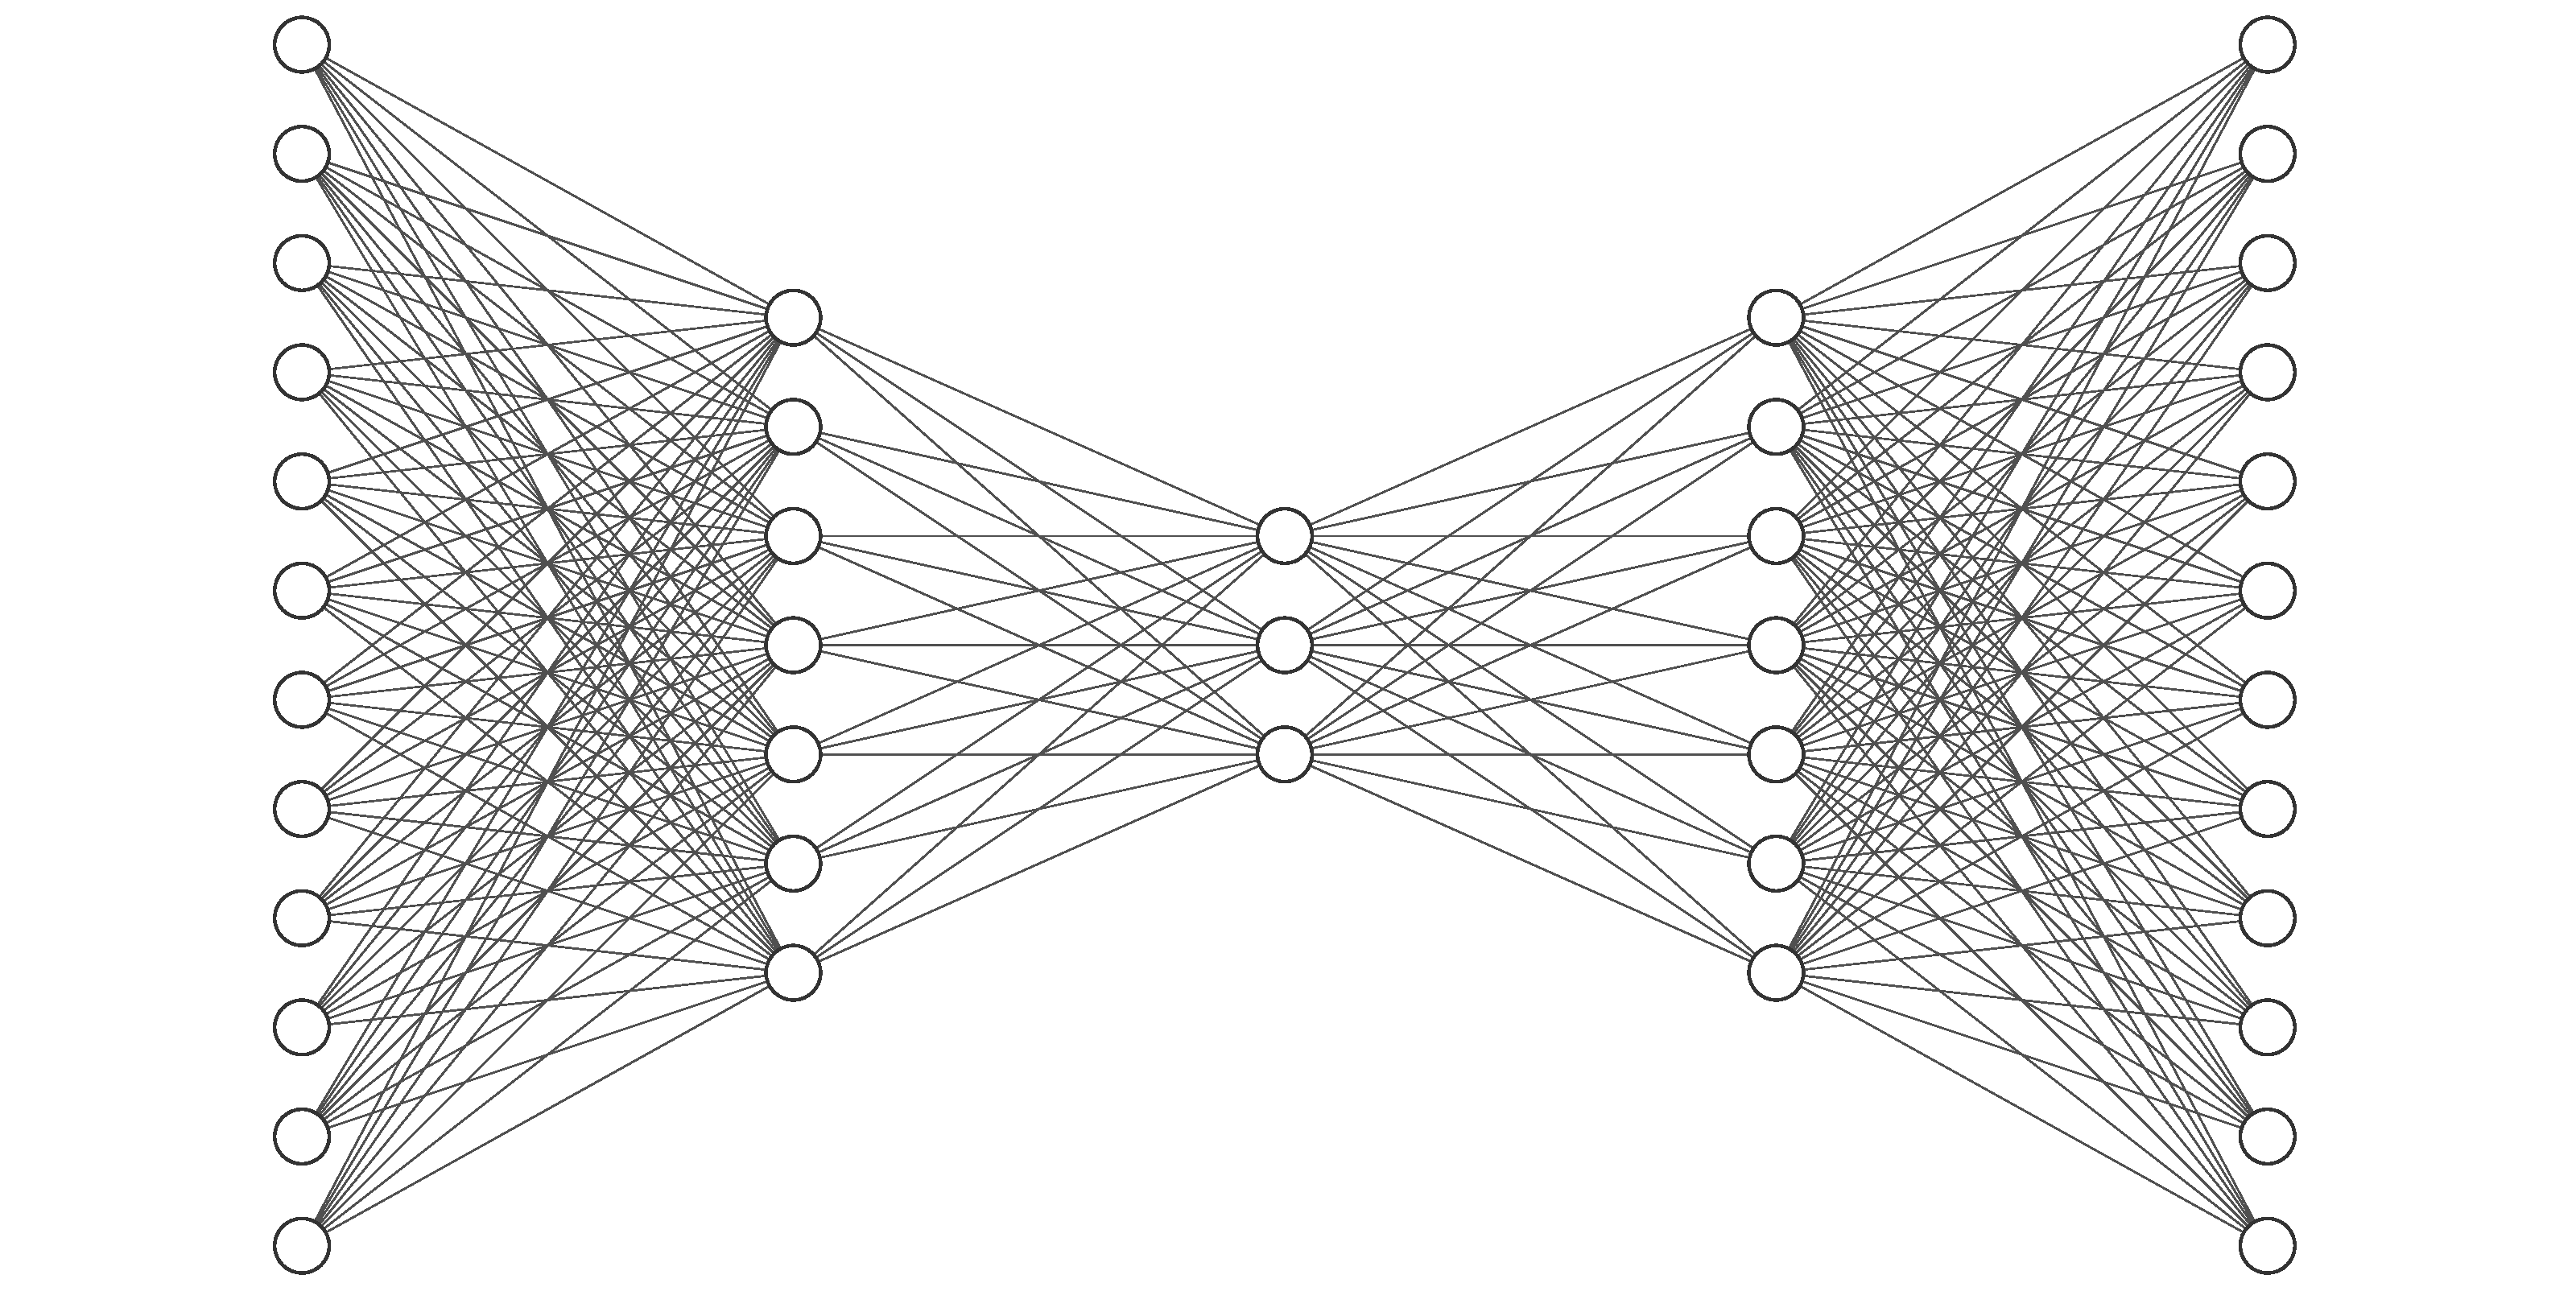
\includegraphics[width=\textwidth]{5_layer_AE.pdf}
		\caption[Schematische Abbildung der Architektur eines Autoencoders]{Gezeigt ist eine schematische Abbildung der Architektur eines Autoencoders. Dieser Autoencoder besitzt fünf Schichten, wobei das \textit{Bottleneck} dreidimensional und die \textit{Input}-Dimension zwölf ist. Das bedeutet, dass ein 12-dimensionaler Inputvektor in der Mitte des Autoencoders durch einen dreidimensionalen Vektor kodiert und anschließend wieder dekodiert werden muss, um zu einer möglichst verlustfreien Rekonstruktion zu gelangen.}
	\end{center}
\end{figure}

\subsection{Variational Autoencoder}
\label{ch:MethodenDerDimRed:modern:VAE}
\nomenclature[Z]{VAE}{Variational Autoencoder}

\subsection{Self-Organizing Maps}
\label{ch:MethodenDerDimRed:modern:SOM}
\nomenclature[Z]{SOM}{Self-Organizing Map}
